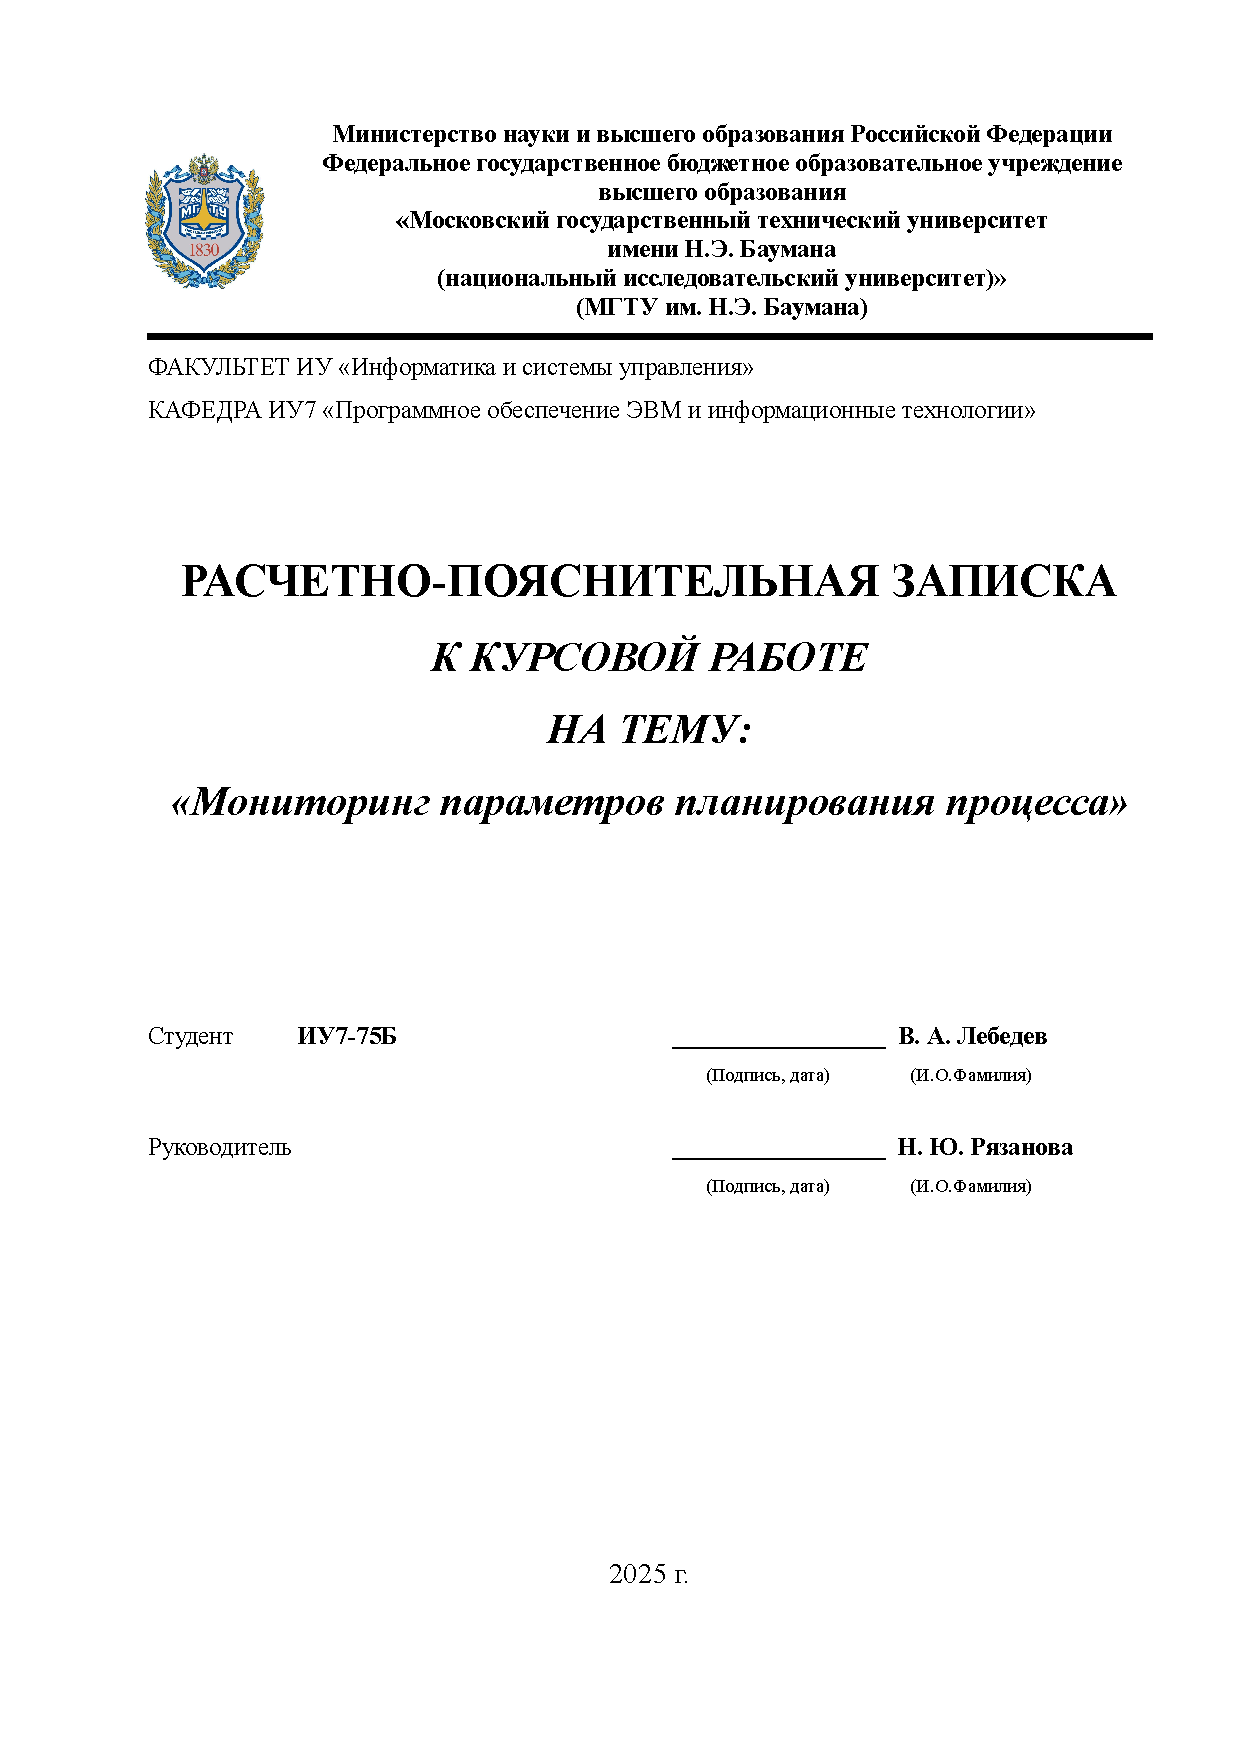
\includepdf[pages={1}]{parts/title.pdf}

\clearpage
~\newpage

\phantomsection
\section*{\centering РЕФЕРАТ}
\addcontentsline{toc}{section}{РЕФЕРАТ}
\setcounter{page}{3}

Расчетно-пояснительная записка \pageref{LastPage} с., \totalfigures\ рис., 1 табл., 3 лист., 7 ист., 1 прил.

Ключевые слова: ВЕБ-СЕРВЕР, PREFORK, PSELECT, МУЛЬТИПЛЕКСИРОВАНИЕ.

Объектом разработки является сервер для отдачи статического содержимого.

Целью работы является разработка сервера для отдачи статического содержимого с диска с использованием архитектуры prefork и системного вызова pselect.

Методы проведения работы: анализ предметной области, проектирование статического сервера, разработка сервера, нагрузочное тестирование, исследование зависимости временных характеристик от числа клиентов.



